\label{chapter:metodo}
\section{Visão geral do método proposto}
   
O sistema computacional proposto será estruturado em forma de boia aquatica, que será composta com microcontroladores, e sensores para análise da água e para a captura ótica, visando adquirir imagens subaquáticas em tempo real. O sistema proposto contará com um módulo de classificação em uma central conectada a boia como pode ser visto na Figura \ref{fig:bigpic}, onde os dados serão processados e exibidos para o usuário final. 
   
%O sistema terá um sensor de captura ótica, que ficará submersos em água, acoplados à uma boia, que terá um conexão sem fio com um celular ou computador.

\begin{figure}[ht]
	\centering
    \caption{\label{fig:bigpic}Visão Geral}
	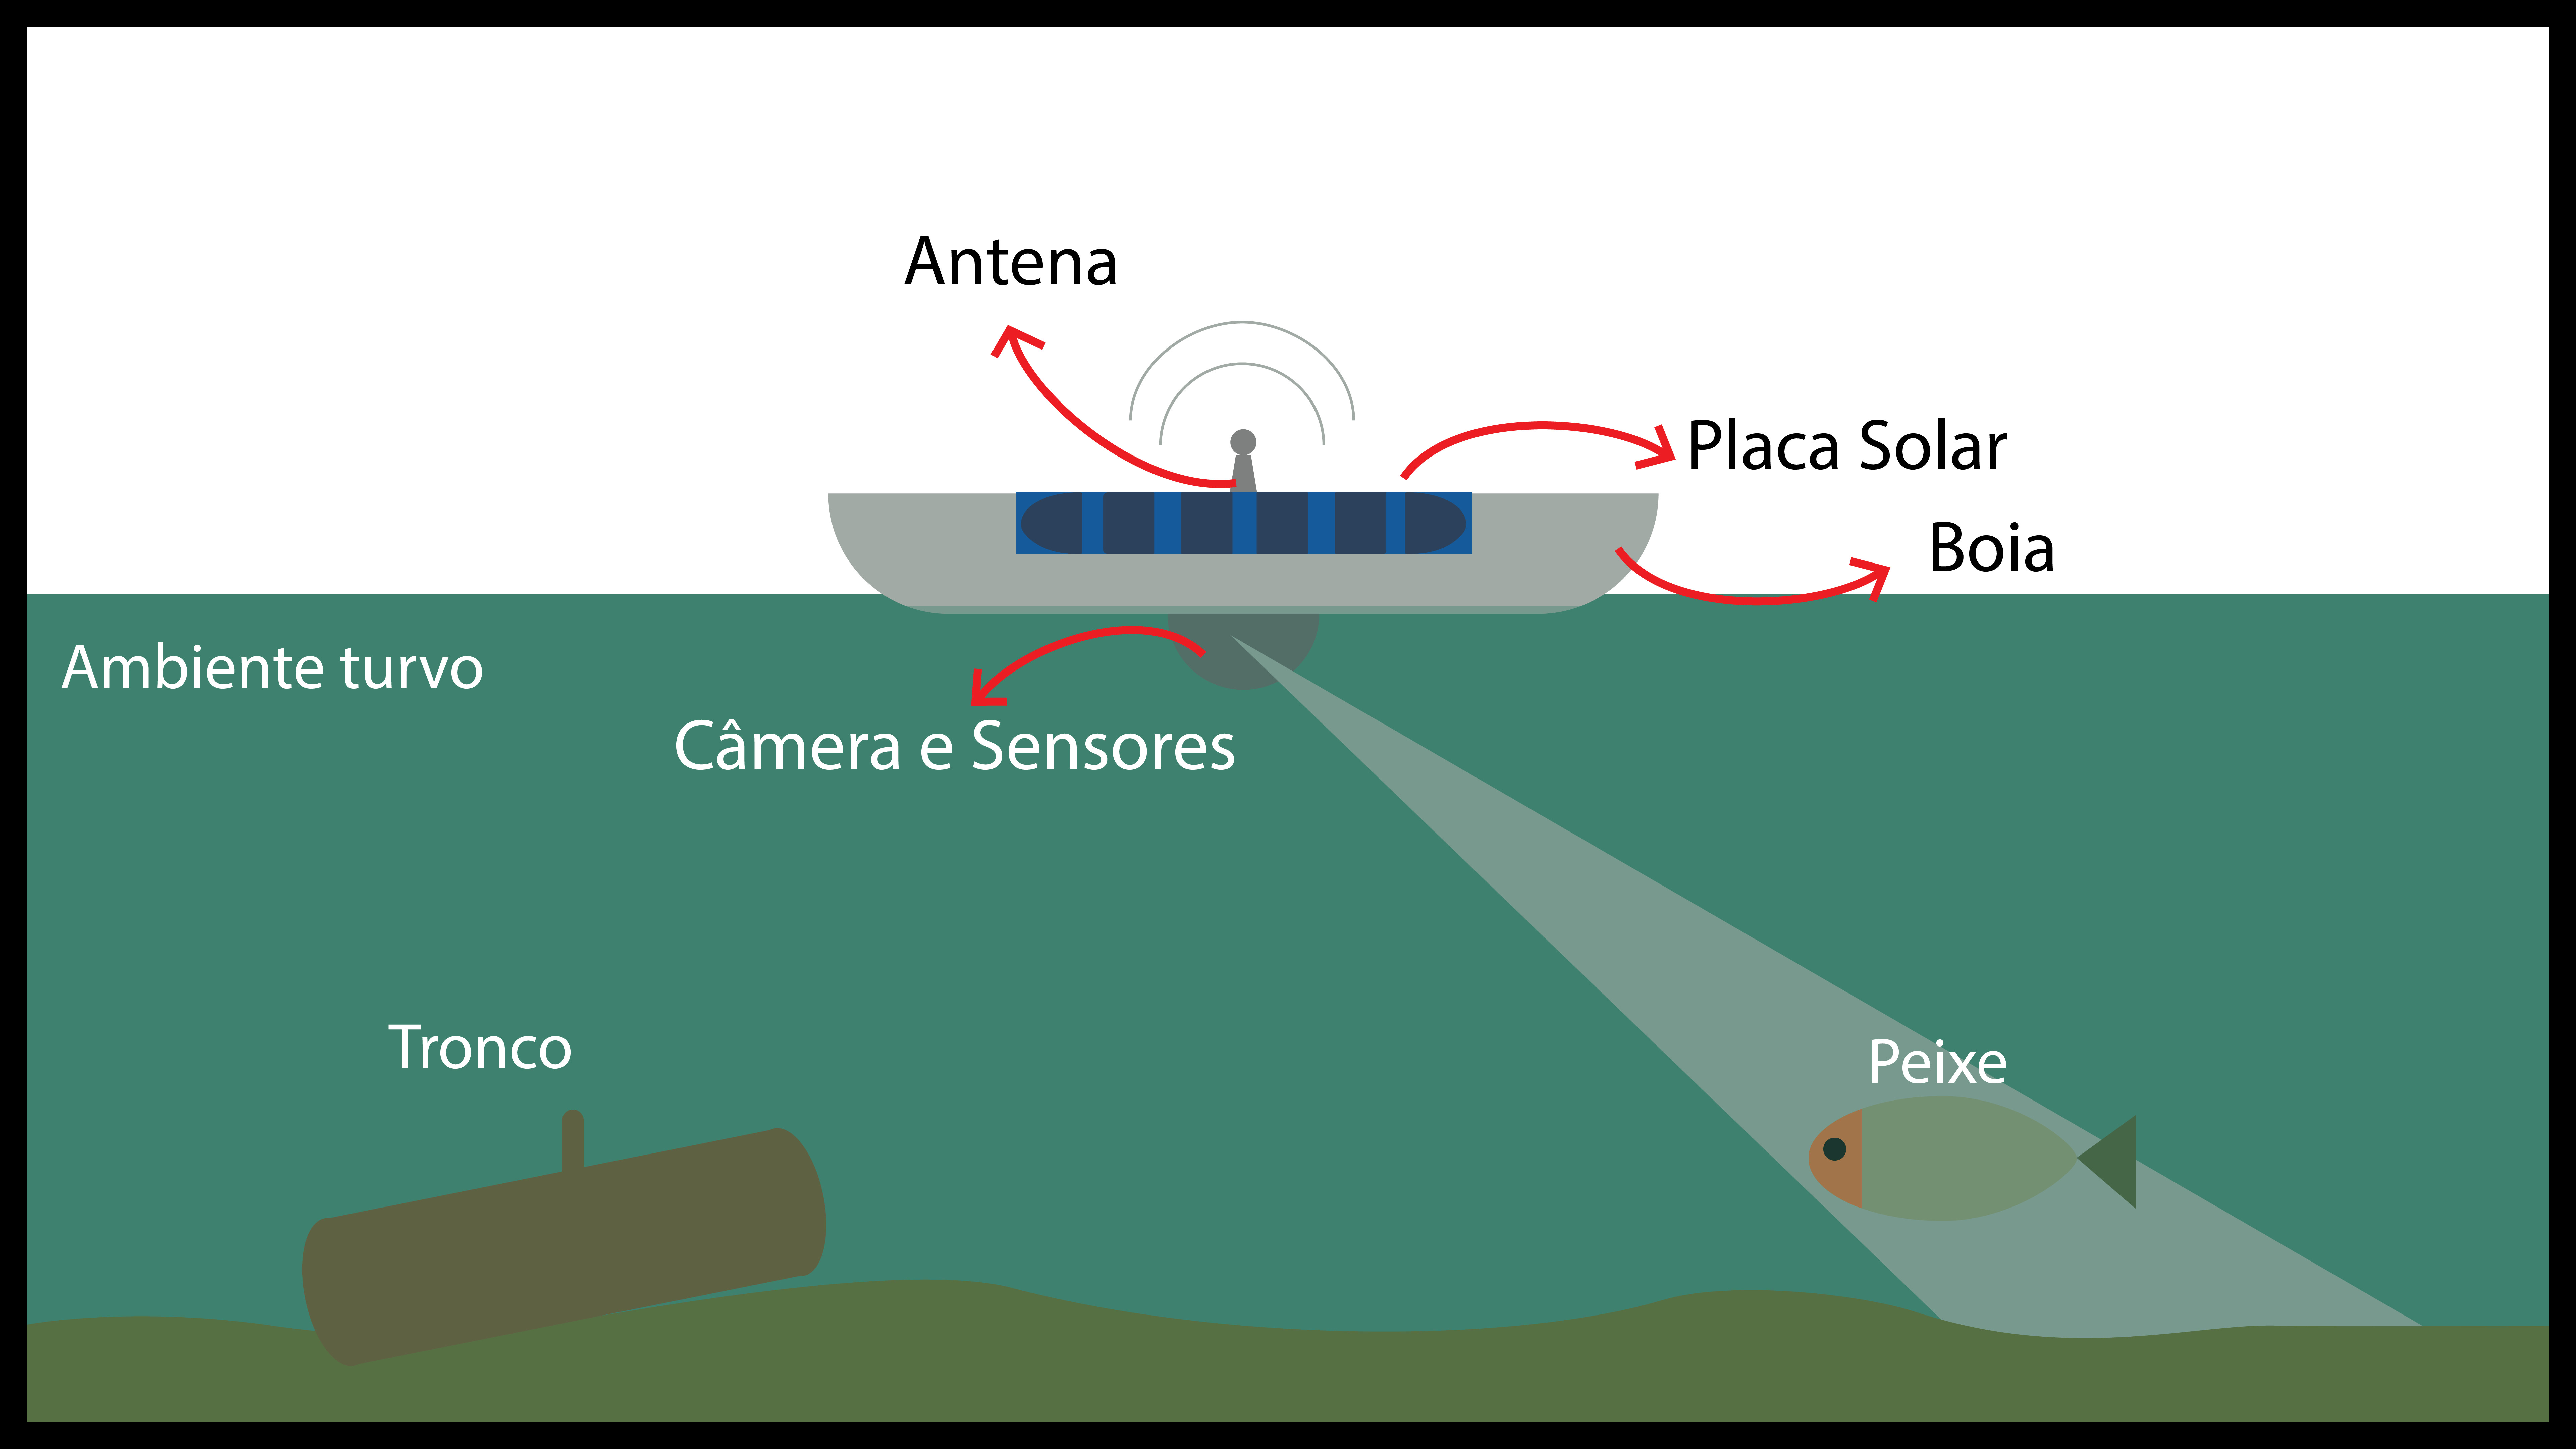
\includegraphics[width = 0.6\textwidth]{resources/bugpicturefloater}
    \legend{Fonte Própria}
\end{figure}

\todo[inline]{Descrever a imagem, na imagem tb não tem a parte da central}

\section{Sistema computacional de suporte a coleta de imagens em ambientes fluviais: Kraken}
%\todo{o que será a boia;
%que sensores irá utilizar;
%como será a conexão com a centra;
%como será a centra;
%falar sobre a possibilidade de adição de sensores;}

O projeto será uma boia que com auxílio de microcontroladores que irão controlar os sistemas integrados ao sistema proposto, como motores e/ou estabilizadores e sensores para detecção de objetos e captura de imagens dentro do ambiente fluvial com alta turbidez, identificando objetos, classificando-os e especulando seu tamanho.

\todo[inline]{O Texto acima está muito similar ao do ínicio modificar e ampliar a descrição de onde o sistema poderá ser utilizado}

A boia conta com auxílio de um módulo de classificação  de imagens que pode ser \textit{modelado} de acordo com a necessidade do ambiente, em especifico neste trabalho iremos adotar o \textit{framework Tensorflow}. A imagem será pré-processada antes de ser enviada ao classificador, isso irá garantir que a imagem esteja em perfeitas condições de classificação.

A utilização de uma plataforma de sistema integrada com uso de microprocessador, contendo várias entradas (digitais e analógicas) irá garantir o suporte para novas extensões como um oxímetro, quer irá medir o nível de oxigênio na água. O uso do microprocessador será o meio para interligar a maioria dos sensores e fará a conexão com a central, garantindo que os dados sejam tratados e enviados ao usuário final.

A central contará com um aplicativo de auxílio, onde serão exibidos os resultados para o usuário, tais como os dados coletados pela boia, garantindo uma entrega rápida de informação. Os dados classificados terão seus tamanhos especulados, e as imagens serão tratadas usando filtros com a biblioteca \textit{OpenCV}. O fluxo do sistema pode ser visto na \autoref{fig:fluxfish}, que descreve como o será o fluxo do sistema.

\todo[inline]{O texto acima está muito confuso, mistura a classificação com as funções da boia, corrigir. Tudo deve se integrar e comunicar está faltando ordem.}

\begin{figure}[ht]
	\caption{\label{fig:fluxfish}  Fluxo de funcionamento do sistema proposto.}
	 \begin{center}
		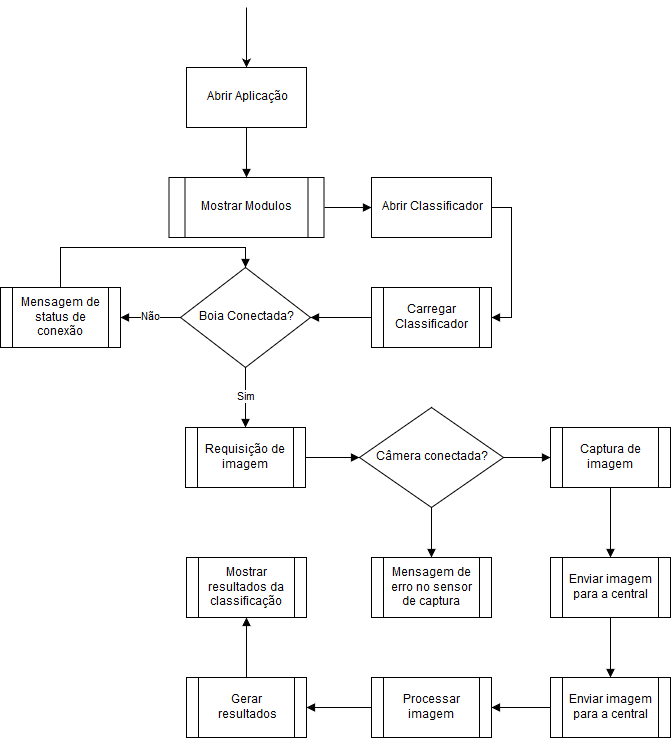
\includegraphics[width = 0.9\textwidth]			{resources/fluxogeral}
    \end{center}
    \legend{Fonte Própria}
\end{figure}

\todo[inline]{O Fluxo deve ser explicado e detalhado o seu funcionamento}


O diagrama de sequência representeado pela \autoref{fig:segkraken} mostra a sequência de interações do sistema, tais como: a interação do usuário com a Central; e da Central com a Boia. As condições caso haja falha nas conexões com os sensores e como proceder caso essas falhas sejam encontrodas.

\begin{figure}[ht]
	\caption{\label{fig:seqkraken}  Diagrama de sequencia do sistema proposto.}
	 \begin{center}
		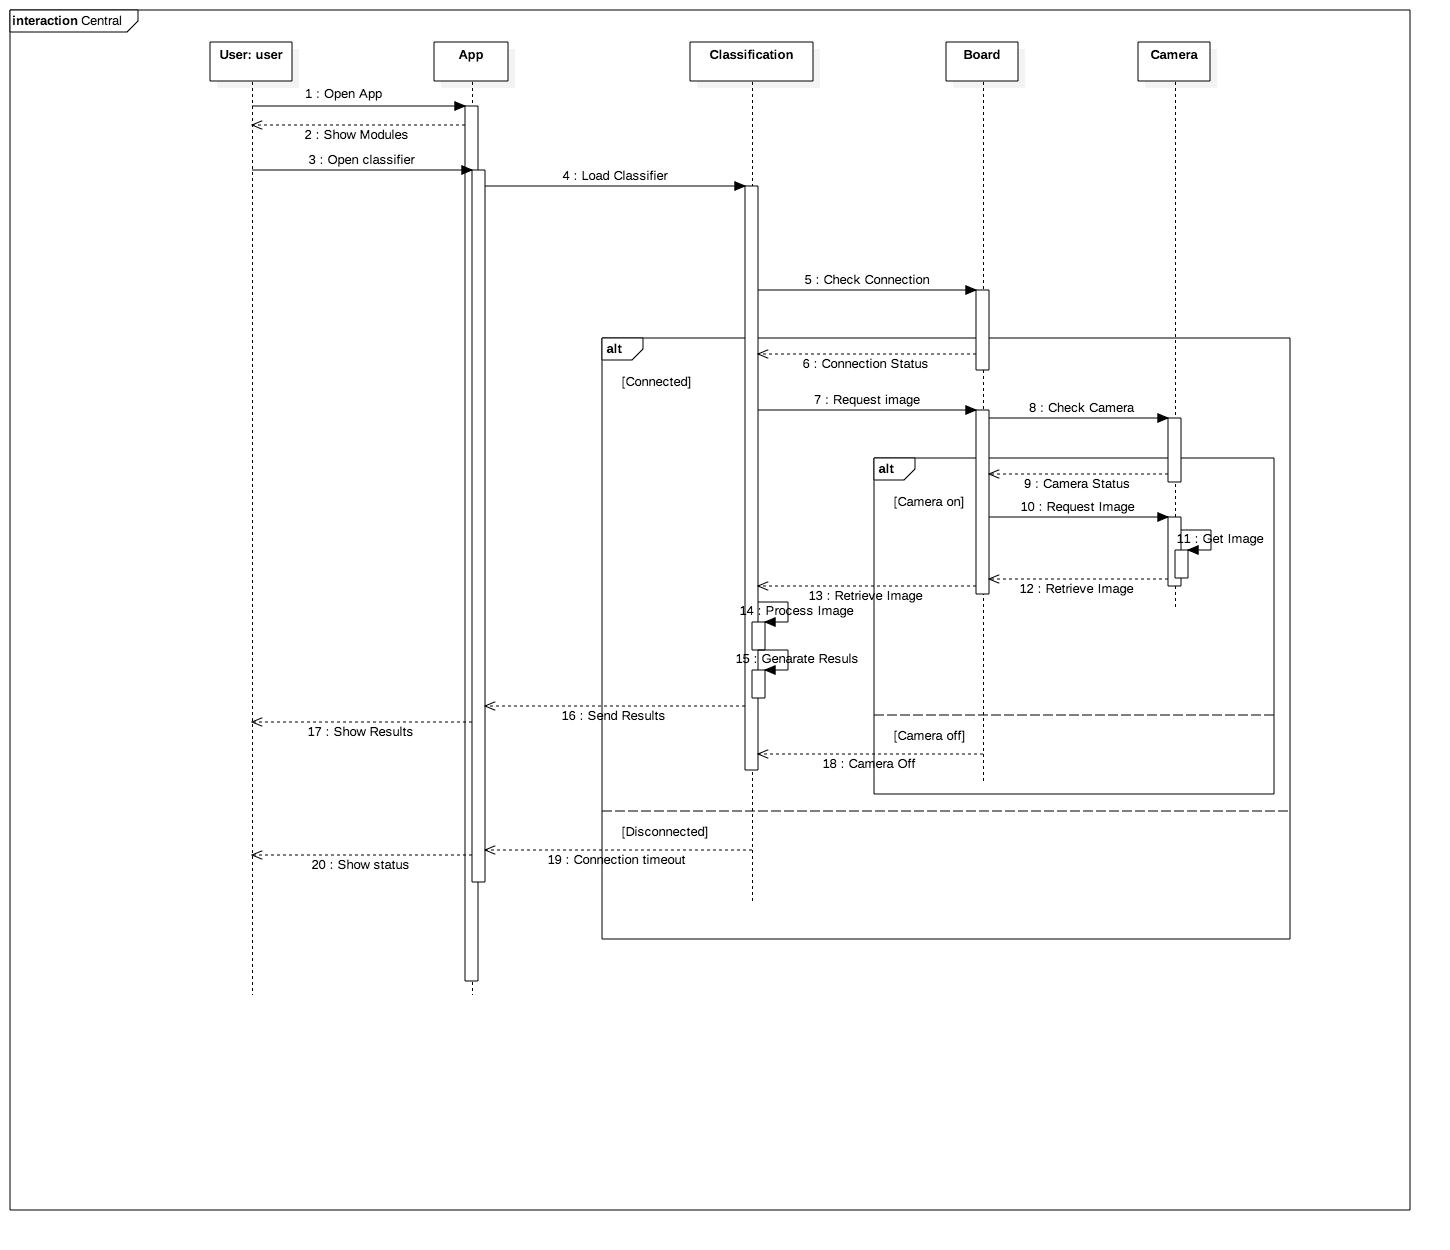
\includegraphics[width = 0.9\textwidth]			{resources/sequencekraken}
    \end{center}
    \legend{Fonte Própria}
\end{figure}

\todo[inline]{As imagens não estão em ordem}

\todo[inline]{O diagrama UML deve ser explicado e detalhado o seu funcionamento}


\section{Analise dos dados na central de processamento}

Após a coleta das imagens, captados pelos sensores de captura as imagens\todo{exemplificar sensores} serão enviadas através de uma rede \textit{Wireless} para a Central, onde serão processados pelo módulo de Classificação que utilizará \textit{OpenCV} para os filtros de pré-processamento afim de melhorar a qualidade da imagem, caso seja necessário, e adequá-las para classificação usando o \textit{Tensorflow}, previamente modelado utilizando \textit{Inception}\todo{Descrever o que é o Inception}, para retreinar as últimas camadas da sua rede neural\todo{Descrever pq isto é feito}. 
Após o processamento da imagem, será gerado um relatório sobre os dados processados dessa imagem, exibindo pro usuário o tamanho especulado\todo{Como o tamanho será calculado} e o resultado da classificação\todo{Qual será o tipo de saida desta classificação?}.

\subsection{Pré processamento}

\todo[inline]{Adicionar texto de instrodução a seção, explicando a razão desta etapa.}
\todo{place-holder}

\subsubsection{Homomorphic filtering}

\todo[inline]{Texto em inglês??????}
The homomorphic filtering is used to correct non uniform illumi- nation and to enhance contrasts in the image. It’s a frequency filtering, preferred to others techniques [4][8] because it corrects non uniform lighting and sharpens the edges at the same time.


\todo{place-holder}\subsubsection{Anisotropic filtering}
\todo[inline]{Texto em inglês??????}
 Anisotropic filtering allows us to simplify image features to improve image segmentation. This filter smooths the image in homogeneous area but preserves edges and enhance them. It is used to smooth textures and reduce artifacts by deleting small edges amplified by homomorphic filtering.


\section{Análise dos sensores}
Com a possibilidade da adição de extensões à Boia, como sensores de medição de oxigenação da água, a necessidade de analise desses é algo pertinente para o desempenho da boia. dada determinada situação onde a água não está com turbidez a utilização de um sensor pode detectar o ambiente e evitar que a central não necessite utilizar os filtros de pré-processamento nas imagens capturadas, melhorando o tempo de classificação.

\todo[inline]{Confuso, a etapa será no futuro, não faz parte do método?}



\section{Construção da Boia}

A estrutura da Boia será baseada na estrutura representada pela  \autoref{fig:shubfloater}, que visa baixo custo, utilizando materiais que podem ser encontrados com facilidade, como canos de PVC para a sustentação dos sensores e placas, tendo grande potencial para extensões ou modificações como alterar a estrutura para adicionar outro tipos de motores.

\begin{figure}[ht]
	\caption{\label{fig:shubfloater}  Estrutura de USV proposto por 
	Shubham.}
	 \begin{center}
		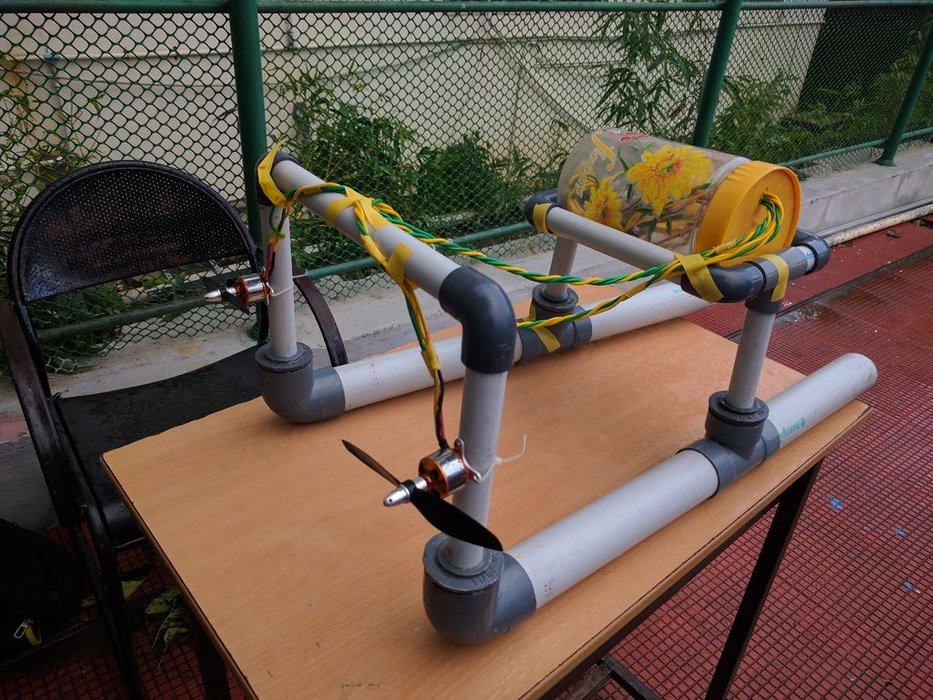
\includegraphics[width = 0.8\textwidth]			{resources/shubhamfloater}
    \end{center}
    \legend{Fonte: http://www.instructables.com/id/Arduino-RC-Amphibious-Rover/}
\end{figure}

\todo[inline]{Os meus comentários sobre está imagem não foram implementados}

\todo[inline]{O ideal nesta parte é vc apresentar os componentes e uma possivel forma de construção e validação do prototipo}

\todo[inline]{Está seção está bem dificil ainda tem muito trabalho a ser feito, sugiro reescrever. Lembrando que cada etap deve alimentar a próxima conforme o fluxo}

%\section{Identificação de Objetos utilizando openCV}
%O método utilizado para nessa primeira fase de identificações consiste nas seguintes etapas. Como mostra a Figura~\ref{fig:fluxfish} 



%\subsection{Pré-processamento}
%O pré-processamento da imagem é feito com a correção de cores, alterando seu sistema de cores de RGB para BGR como pode ser visto na figura~\ref{fig:fishp1}. 
%\begin{figure}[H]
%	\caption{\label{fig:fishp1} Alteração do sistema de cores para RGB}
%	\centering
%		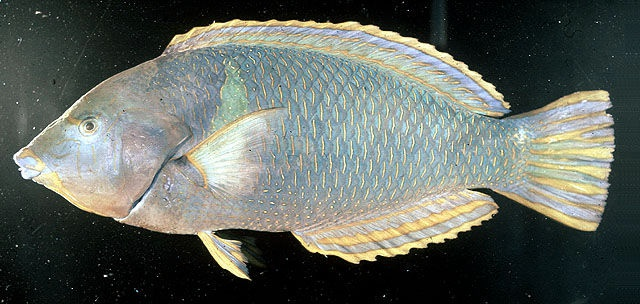
\includegraphics[width = 0.4\textwidth]			{fishes/fish_P1}
 %   \legend{Fonte Própria}
%\end{figure} 
%Para remoção de ruídos um filtro Gaussiano com outra modificação no sistema de cores é aplicado, facilitando a identificação de alguns pontos na imagem. o resultado pode ser visto na figura~\ref{fig:fishp2} 
%\begin{figure}[H]
%	\caption{\label{fig:fishp2} Aplicação de filtro Gaussiano e alteração do sistema de cores para HSV}
%	\centering
%		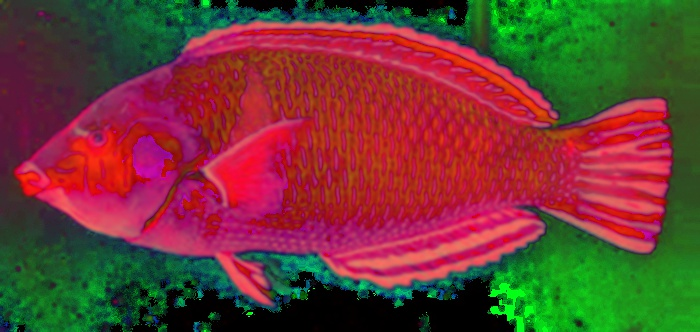
\includegraphics[width = 0.4\textwidth]			{fishes/fish_P2}
 %   \legend{Fonte Própria}
%\end{figure} 

%Em seguida a imagem deve ser livradas de alguns ruídos, assim um filtro gaussiano e conversão do sistema de cores serão aplicados. Resultado na Figura~\ref{fig:fishp2} 


%\subsection{Segmentação e identificação de objetos}
%A máscara de segmentação é baseada nos níveis de cores encontrados na imagem. Dois filtros são criados com espectros de cores diferentes e em seguida mesclados. . o resultado pode ser visto na figura~\ref{fig:fishp3_mask1}, a figura~\ref{fig:fishp5} mostra a exclusão de segmentos não necessários.
%\begin{figure}[H]
%	\caption{\label{fig:fishp3_mask1} Extração das máscaras}
%	\centering
%		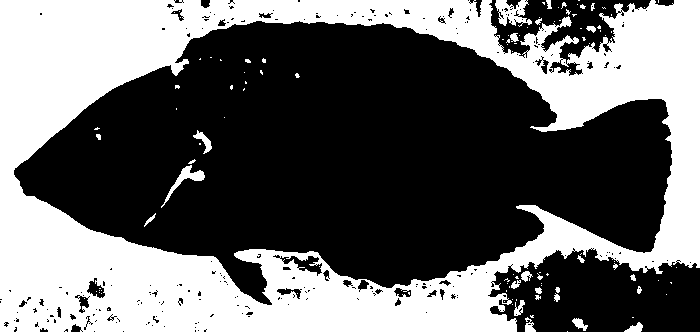
\includegraphics[width = 0.4\textwidth]			{fishes/fish_P3_mask1}
%    \legend{Fonte Própria}
%\end{figure}
%\begin{figure}[ht]
%	\caption{\label{fig:fishp5} Exclusão de segmentos}
%	\centering
%		
\includegraphics[width = 0.4\textwidth]			{fishes/fish_P5_mask_fishes}
 %   \legend{Fonte Própria}
%\end{figure} 

%A identificação de objetos na imagem é realizada através da identificação dos maiores pontos encontrados nas máscaras de segmentação, então esses são circulados, gerando a imagem de saída.
%\begin{figure}[H]
%	\caption{\label{fig:fishp5} Saída}
%	 \centering
%		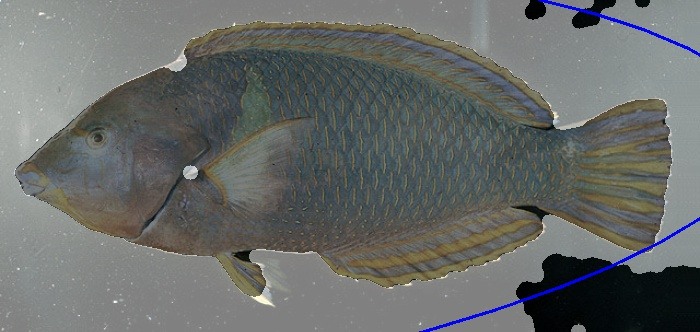
\includegraphics[width = 0.6\textwidth]			{fishes/fish_P7}
%    \legend{Fonte Própria}
%\end{figure}



